%We report on our experience of applying the proposed design and implementation
%to the mechanization of language metatheories.

%To demonstrate the applicability of our design and implementation, we
%conduct two case studies.


\noindentparagraph{Type safety of STLCs.}

The first case study is the mechanization of the type safety theorem of
STLC and those of its extensions,
which has been occurring in the examples in this paper.
The code base is ported from Software Foundations~\cite{sf-pl}.
%
The linguistic nature of our approach allows us to retain a programming
style similar to the original proofs in Software Foundations.

The base STLC family consists of \textasciitilde360~LOC,
about the same as an STLC development not using \Lang.
%
Lines of code in each of the four derived families
($\mathrm{Y}$, $\times$, $+$, and $\mu$ in the Venn diagram)
vary from 100 to 250,
largely depending on how many constructors they add to the inductive types.
Without \Lang, the same STLC code would have to be duplicated for each feature.

\begingroup
\small
\renewcommand*{\arraystretch}{0.75}

\def\CircFix{(135:0.707cm) circle (1.5cm)}
\def\CircProd{(45:0.707cm) circle (1.5cm)}
\def\CircIsorec{(-45:0.707cm) circle (1.5cm)}
\def\CircSum{(-135:0.707cm) circle (1.5cm)}

\definecolor{FixColor}{HTML}{FF9966}
\definecolor{ProdColor}{HTML}{66CCFF}
\definecolor{SumColor}{HTML}{FFFF66}
\definecolor{IsorecColor}{HTML}{FF6699}

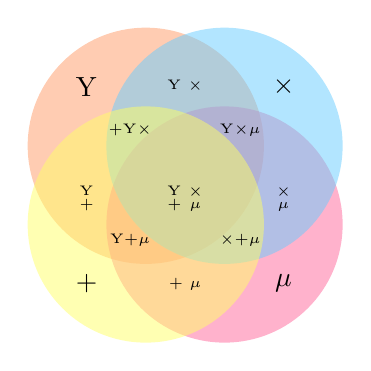
\begin{tikzpicture}
    \begin{scope}[shift={(0cm,-0cm)}, fill opacity=0.50]
        \fill[FixColor] \CircFix;
        \fill[IsorecColor] \CircIsorec;
        \fill[ProdColor] \CircProd;
        \fill[SumColor] \CircSum;
%       \draw \CircFix;
%       \draw \CircIsorec;
%       \draw \CircProd;
%       \draw \CircSum;
    \end{scope}

    \node at (0: 0) {%
        \begin{minipage}{1cm}\tiny
        \[\begin{array}{@{}c@{\ }c@{}}
            \mathrm{Y} & \times\\ + & \mu
        \end{array}\]
        \end{minipage}
    };
    \node at (-180: 1.25cm) {%
        \begin{minipage}{1cm}\tiny
        \[\begin{array}{@{}c@{}}
            \mathrm{Y}\\ +
        \end{array}\]
        \end{minipage}
    };
    \node at (0: 1.25cm) {%
        \begin{minipage}{1cm}\tiny
        \[\begin{array}{@{}c@{}}
            \times\\ \mu
        \end{array}\]
        \end{minipage}
    };
    \node at (90: 1.26cm) {\tiny$\mathrm{Y}\ \times$};
    \node at (-90: 1.26cm) {\tiny$+\ \mu$};
    \node at (135: 1.768cm) {$\mathrm{Y}$};
    \node at (-135: 1.768cm) {$+$};
    \node at (45: 1.768cm) {$\times$};
    \node at (-45: 1.768cm) {$\mu$};
    \node at (45: 0.988cm) {\tiny$\mathrm{Y}$$\times$$\mu$};
    \node at (-45: 0.988cm) {\tiny$\times$$+$$\mu$};
    \node at (-135: 0.988cm) {\tiny$\mathrm{Y}$$+$$\mu$};
    \node at (135: 0.988cm) {\tiny$+$$\mathrm{Y}$$\times$};

\end{tikzpicture}
\endgroup

Using individual families to organize the mechanization of individual
language features leads to a modular design that also facilitates code reuse.
%
Individually developed features can be easily composed (as mixins) to
form new STLC variants (e.g., $\mathrm{Y}$$+$$\mu$).
%
Such a feature composition often requires only a few lines of code.

Composing features can lead to \emph{feature interactions}~\cite{batory2011feature}:
features working correctly in isolation may require coordination when composed.
For example, composing $\times$ and $\mu$  %\lsti{STLCIsorec} and \lsti{STLCProd}
(\cref{fig:stlc-isorec-prod}) creates an obligation to extend \lsti{tysubst} to
handle \lsti{ty_prod}, which the type-checker enforces.
%
Composing contradictory features (e.g., a fixpoints construct and a strong
normalization theorem) would lead to unprovable proof obligations.

Elimination of inductive types defined via \lsti{FInductive} is
mostly via the \lsti{FRecursion} and \lsti{FInduction} commands.
An exception is a handful of trivial ``inversion lemmas''.
For example, consider the lemma \lsti!\forall t, \neg step tm_true t!
stating that \lsti!tm_true! is irreducible.
If \lsti{step} were an ordinary inductive type, then it could be proved in Coq
simply by \lsti{intros t H; inversion H}.
But \lsti{step} is extensible. So one way to prove the lemma is
by \lsti{FInduction} on \lsti{step} and verifying that
a derived family does not accidentally make \lsti{tm_true} reducible.
%lemma still holds in derived families that add new constructors to \lsti{step}.
%
We observe that it is lighter-weight to use overriding (\cref{sec:override}) instead:
the programmer can specify that the proof of the lemma should be overridden
in any derived family that further binds \lsti{step},
and in return, they are permitted to treat \lsti{step} as an ordinary
inductive type in the proof and thus use \lsti{inversion} to prove it.
The plugin then automatically tries the same proof script in a derived
family to override the proof. Although proof scripts rather
than proof terms are reused, this practice seems justified
by the triviality of the lemmas and the terseness of the proof scripts.

%The current plugin implementation does not yet support
%mutually inductive types or mutual induction, which are
%useful for modeling languages much more complex than STLCs.
%However,
%we believe accommodating mutually inductive types does
%not pose theoretical challenges.

% I think the following is a bit weird ... not enough quantative and not enough qualititive
% When programming in a direct style, before using \Lang, the STLC base module 
% will take around 350LOCs, and STLC with one feature is around 400 LOCs, because
% it requires to repeat the definition of the STLC base definition. It will take 
% more space when we add more features into STLC.

% After using \Lang, the 
% STLC base family also take about 350 LOCs. However, one feature as children family takes only about 100~250 LOCs. What's more, the mixin of two features usually only take 1~20 LOCs.
%When programming in a direct style, before using \Lang, the STLC base module will take around 350 LOCs while using \Lang, the STLC base family takes about same amount of the code. 

%However, without \Lang, STLC with one feature will require around 400 LOCs as the definition of STLC base is repeated. On the other hand, using \Lang, each feature as extended family only requires ranging from 100~250 LOCs. What's more, without \Lang, STLC with multiple features will require more and more while using \Lang's mixin feature, tens of LOCs is enough.

\noindentparagraph{Abstract interpreters for imperative languages.}

Our second case study is a mechanization of abstract interpreters
for simple imperative languages.
In addition to a soundness proof, this case study produces abstract
interpreters that are directly ready for program extraction.

The code is organized into four families.
A base family \lsti{Imp} (\textasciitilde 200~LOC) defines via \lsti{FInductive} the abstract
syntax of a while-language with pure expressions and impure statements.
The semantics is given by an interpreter defined as a CEK-style abstract
machine~\cite{felleisen1986control} and parameterized by a fuel value.
Family \lsti{Imp} defines the interpreter via \lsti{FRecursion}.

A second family \lsti{ImpGAI} (\textasciitilde 550~LOC) extends \lsti{Imp}.
It exports a generic framework for deriving
abstract interpreters with partial-correctness guarantees.
Soundness of the abstract interpreter, \lsti{analyze},
is stated with respect to the interpreter, \lsti{eval}, inherited from \lsti{Imp}.
The theorem says that the abstraction relation \lsti{RState} over a
concrete state~\lsti{S} and an abstract state~\lsti{absS} is preserved
by the analysis:

\begin{centered}
\begin{minipage}{.91\textwidth}
\begin{lstlisting}[basicstyle=\fontsize{8.25}{9}\ttfamily]
\forall stmt fuel S absS, RState S absS -> RState (eval fuel stmt S) (analyze fuel stmt absS)
\end{lstlisting}
\end{minipage}
\end{centered}

\begin{wrapfigure}[13]{r}{0.138\textwidth}
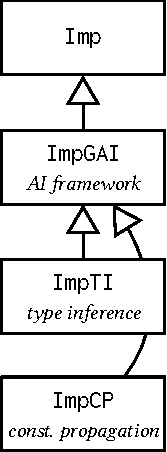
\includegraphics[scale=.68]{graphics/ai-casestudy.pdf}
\end{wrapfigure}

\noindent
\lsti{analyze} is defined via \lsti{FRecursion}, and the soundness theorem
is proved via \lsti{FInduction}.
This family leaves fields representing the abstract domain, the
abstraction relation, monotonicity of transfer functions, etc.\ 
largely unspecified or unproven---a derived family can further bind
these ``parameters'' by overriding appropriate fields (and also possibly
extend the abstract syntax), to create a sound, runnable abstract
interpreter for a (possibly extended) while-language.
%\EDJ{It is not very relaxed. Currently everything is using a dicionary as memory model and stick with that. The abstract value for each expression is the one *really* unspecified.}

The next two families then extend \lsti{ImpGAI}.
Family \lsti{ImpTI} (\textasciitilde200~LOC) is an abstract
interpreter that does type inference~\cite{cousot1997types}.
Family \lsti{ImpCP} (\textasciitilde300~LOC) extends the abstract syntax
with natural-number arithmetic,
and further binds the generic abstract interpreter to perform constant propagation.
%
An alternative to \Lang would be to define \lsti{ImpGAI} as a functor parameterized
by the abstract domain and such. But it would prevent \lsti{ImpCP} from reusing
the code and proofs in \lsti{ImpGAI}, because \lsti{ImpCP} involves extending
inductive types with new constructors.

Our implementation of family polymorphism is compatible with Coq's
program extraction feature.
We extract the two verified abstract interpreters to OCaml.
Testing the extracted program over simple queries returns expected results.
%\rD{What were the results of testing the extracted abstract interpreters? I don't expect much in the way of performance, but did they return the correct results? What sorts of benchmarks did you use?}

We note that \Lang cannot yet allow the expression of two derived abstract
interpreters nested within the same family.
Work on nested inheritance~\cite{ncm2004,zm2017} points to a direction
to further increase the expressive power of our language design.

%If not using \Lang, we can construct \lsti{Imp}, \lsti{ImpGAI} and \lsti{ImpTI} in a similar way---but \lsti{Imp} is now a module instead of a family, \lsti{ImpGAI} is now a functor instead of a family with overridable fields, and \lsti{ImpTI} is a concrete instantiation of the functor \lsti{ImpGAI}. However, \lsti{ImpCP} cannot reuse the above framework as it extends syntax with natural numbers. Thus \lsti{ImpCP} will require repeating a large amount of definitions, and it alone will needs about 900~LOCs.

In addition to the two case studies above, we also use extensible
inductive types for modeling extensible context-free grammars and derive
decision procedures for language membership.
%\EDJ{I will suggest change to ``and derive decision procedures for them (based on naive parsing by enumeration)''.}

%\cref{sec:coqexample-stlc}
%\cref{sec:coqexample-analysis}
%\cref{sec:coqexample-parser}